%---------------------------------------------------------------------
%
%                          Capítulo 5
%
%---------------------------------------------------------------------

\chapter{Text2LSE}


En este capítulo se muestra el desarrollo que se ha realizado a lo largo de este proyecto. Text2LSE es una aplicación web (ver Figura~\ref {fig: imgWebText2LSE}) que permite traducir textos escritos en castellano a LSE en formato texto, vídeo e imagen en tiempo real. Text2LSE es pública, y se puede acceder a ella desde la siguiente url: 

\begin{shaded}
	\url{https://holstein.fdi.ucm.es/tfg-text2lse }	
\end{shaded}

Está basada en servicios web, los cuales están disponibles para todo el mundo de manera gratuita. Los vídeos e imágenes utilizados en la traducción a LSE son los recursos ofrecidos en el catálogo de LSE de ARASAAC. \\

En la sección 5.1 se muestra la arquitectura de la aplicación web y cómo se comunica ésta con los servicios web. En la sección 5.2 se explican en profundidad los servicios web desarrollados, tanto los utilizados en la aplicación web, como los desarrollados para aumentar las posibilidades de obtención de información para futuros desarrolladores. A continuación, en la sección 5.3 se detalla la aplicación web, tanto el diseño como su funcionalidad. \\


\begin{figure}[]
	\centering
	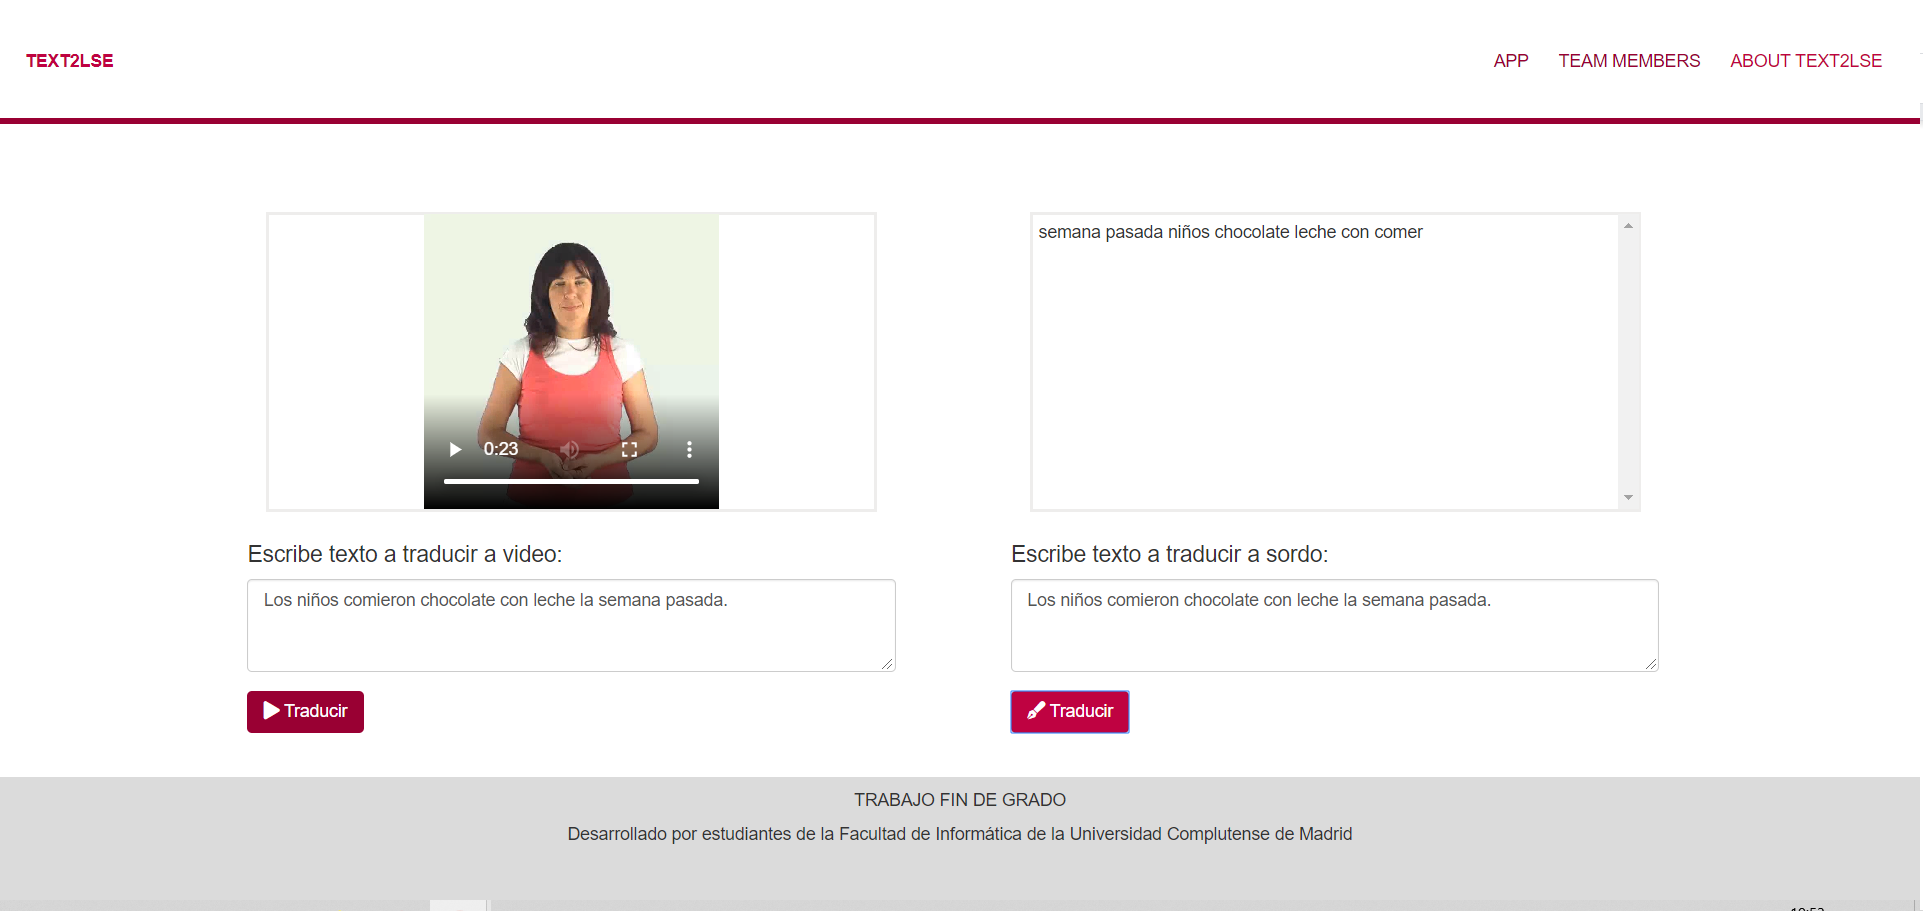
\includegraphics[width=1\textwidth]{Imagenes/Fuentes/Text2LSE/WebText2LSE.png}
	\caption{Aplicación web Text2LSE }
	\label {fig: imgWebText2LSE}
\end{figure}

%-------------------------------------------------------------------
\section{Arquitectura}
%-------------------------------------------------------------------
\label{cap4:sec:Arquitectura}

Text2LSE es una aplicación de traducción de castellano a LSE basada en servicios web, de manera que el código desarrollado sea fácilmente reutilizable. La arquitectura utilizada para el desarrollo de este proyecto es la arquitectura de cliente-servidor, es decir, un cliente muestra una web, la cual hace peticiones al servidor, que almacena los servicios web y devuelve la respuesta al cliente.\\

Se ha optado por desarrollar una aplicación web debido a que ésta es accesible desde cualquier dispositivo que disponga de un navegador, ya sea un teléfono móvil, una tablet o un ordenador, sean de la marca y tamaño que sean. Para que se pueda ver de manera correcta en todos esos dispositivos, la aplicación web se ha desarrollado siguiendo un diseño responsive, es decir, que su visualización se adapte dependiendo de las dimensiones de la pantalla del dispositivo desde el cual se esté accediendo.\\

La aplicación web ha sido desarrollada en html, css y javascript.\\

Respecto a la parte del servidor, se han desarrollado siete servicios web distintos: dos para devolver de manera rápida el vídeo y la imagen en LSE de una sola palabra, otro para devolver el texto traducido a texto en LSE, dos para devolver el texto LSE para vídeos e imágenes y otros dos para devolver el texto traducido a video e imágenes en LSE. \\

Se ha utilizado un proxy inverso para poder acceder tanto a la página web como a los servicios web a través desde un mismo punto de acceso. Un Proxy inverso es un método de redireccionamiento del tráfico a partes específicas de una infraestructura concreta\citep*{proxyInverso}. Las principales finalidades para las que se usa este tipo de servidores son:

\begin{itemize}
	
	\item \textbf{Anonimización:} el proxy recibe todas las llamadas al servidor y se encarga de filtrarlas y redirigirlas como se haya configurado previamente. De esta manera, desde fuera del servidor no se va a poder obtener ningún tipo de información del servidor ni de los servicios que estén en él, solo se podrá obtener información del proxy.
	
	\item \textbf{Protección y cifrado:} al utilizar un proxy inverso se tiene la posibilidad de instalar sistemas de control y filtros de paquetes que protegen al servidor, aumentando así la seguridad del sistema.
	
	\item \textbf{Balanceo de carga:} permite redirigir las distintas solicitudes entrantes por varios servidores, permitiendo repartir la carga de trabajo para no sobrecargar ningún servidor o equilibrar la carga en el caso de que falle uno de ellos.
	
	\item \textbf{Caché:} el proxy se puede configurar para que sea capaz de almacenar las respuestas del servidor temporalmente para ofrecer una mayor velocidad de respuesta. De esta forma, si se recibe una solicitud cuya respuesta la tiene almacenada el proxy en su caché, se manda la respuesta de manera inmediata haciendo que no reciba tanta carga de procedimiento el back-end.
	
	\item \textbf{Compresión:} un proxy inverso también se puede utilizar como compresor de datos, tanto entrantes como salientes.
	
\end{itemize}

En este proyecto, se ha configurado el servidor Nginx como servidor proxy inverso con el fin de redirigir las distintas solicitudes al servidor correspondientes. Se han especificado una serie de rutas para diferenciar qué llamadas de usuario redireccionar a la página web y cuáles a los servicios web. Esta estructura se puede observar en la Figura~\ref {fig: imgProxy}.

\begin{figure}[]
	\centering
	
	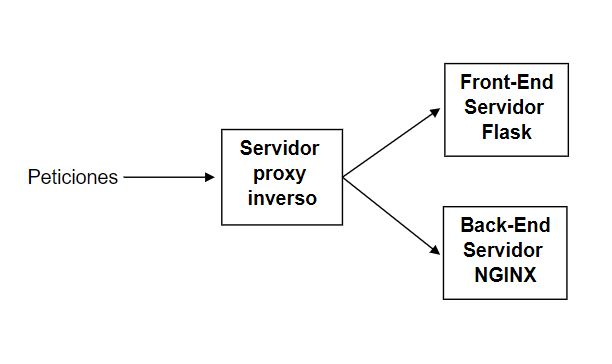
\includegraphics[width=1\textwidth]{Imagenes/Fuentes/Text2LSE/proxy.jpg}
	\caption{Esquema Proxy Inverso}
	\label {fig: imgProxy}
\end{figure}

\section{Back-End}

En esta sección se explican con detalle los servicios web desarrollados, su implementación y cómo utilizan de los recursos LSE de ARASAAC. La API donde están estos servicios es pública\footnote{\url{https://holstein.fdi.ucm.es/tfg-text2lse}} y en los siguientes apartados se indica la URL para acceder a cada servicio.


\subsection{Recursos LSE}

Todas las imágenes y vídeos LSE se han obtenido del catálogo de recursos de ARASAAC\footnote{\url{http://www.http://www.arasaac.org/descargas.php}}, y se almacenan en el propio servidor holstein. Los servicios de traducción de palabra a vídeo LSE y a imagen LSE permiten obtener estos recursos mediante una llamada GET, como se explica a continuación.

\subsection{Servicio web de traducción de palabra a vídeo LSE }

Este servicio permite obtener el video del signo en LSE correspondiente a una palabra en lenguaje natural. Los videos utilizados en este servicio provienen del catálogo de vídeos de LSE de la web de ARASAAC\footnote{\url{http://www.arasaac.org/videos_lse.php}}. Para poder acceder a este servicio, se debe hacer una llamada GET a la API,  indicando la palabra que se desea traducir a LSE de la siguiente forma:\\

\begin{shaded}
	\url{https://holstein.fdi.ucm.es/tfg-text2lse/video/<palabra> }	
\end{shaded}

En el parámetro \textit{``palabra''} se debe indicar la palabra para la que se desea obtener su traducción en LSE. \\

En caso de que se encuentre el vídeo de la palabra buscada, este servicio devuelve el vídeo en formato mp4. En caso de que no se encuentre, devuelve un vídeo de error en formato .mp4. Este flujo lo podemos observar en la Figura~\ref {fig: imgFlujo1palabraText2LSE}. \\

Por ejemplo, para obtener el vídeo en LSE de la palabra \textit{``agua''} se debe realizar la siguiente llamada:

\begin{shaded}
	\url{https://holstein.fdi.ucm.es/tfg-text2lse/video/agua }	
\end{shaded}


\begin{figure}[]
	\centering
	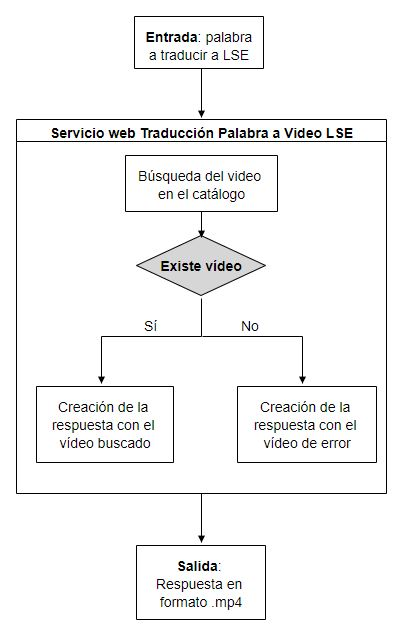
\includegraphics[width=0.7\textwidth]{Imagenes/Fuentes/Text2LSE/FlujoVideo1palabra.jpg}
	\caption{Flujo del servicio de Traducción de una palabra a vídeo en LSE}
	\label {fig: imgFlujo1palabraText2LSE}
\end{figure}

\subsection{Servicio web de traducción de palabra a imagen LSE }

Este servicio permite obtener la imagen del signo en LSE correspondiente a una palabra en lenguaje natural. Las imágenes utilizadas en este servicio provienen del catálogo de imágenes de LSE de la web de ARASAAC\footnote{\url{http://www.arasaac.org/signos_lse_color.php}}. Para poder acceder a este servicio, se debe hacer una llamada GET a la API,  indicando la palabra que se desea traducir a LSE de la siguiente forma:\\

\begin{shaded}
	\url{https://holstein.fdi.ucm.es/tfg-text2lse/imagen/<palabra> }	
\end{shaded}

En el parámetro \textit{``palabra''} se debe indicar la palabra de la que se desea obtener su traducción en LSE. \\

En caso de que se encuentre la imagen de la palabra buscada, este servicio devuelve la imagen en formato .jpg. En caso de que no se encuentre, devuelve una imagen de error en formato .jpg (Figura~\ref {fig: imgError}). Este flujo lo podemos observar en la Figura~\ref {fig: imgFlujo1palabraImagenText2LSE}. \\

Por ejemplo, para obtener la imagen en LSE de la palabra \textit{``coche''} se debe realizar la siguiente llamada:

\begin{shaded}
	\url{https://holstein.fdi.ucm.es/tfg-text2lse/imagen/coche }	
\end{shaded}

La respuesta a la llamada del ejemplo devolverá la imagen de la Figura~\ref {fig: imgCoche}.

\begin{figure}[]
	\centering
	
\includegraphics[width=0.5\textwidth]{Imagenes/Fuentes/Text2LSE/imgError.jpg}
	\caption{Imagen de error devuelta en la traducción de una palabra a LSE}
	\label {fig: imgError}
\end{figure}

\begin{figure}[]
	\centering
	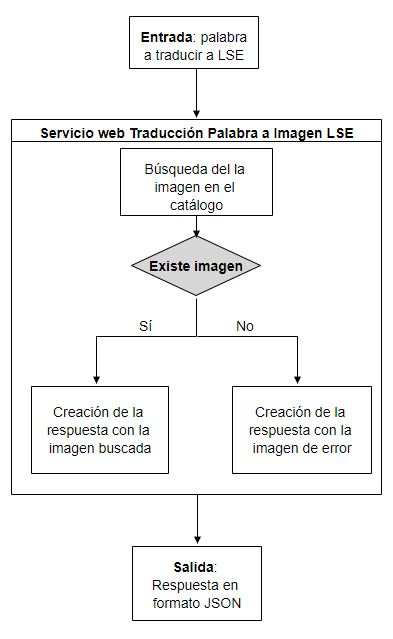
\includegraphics[width=0.7\textwidth]{Imagenes/Fuentes/Text2LSE/FlujoImagen1palabra.jpg}
	\caption{Flujo del servicio de Traducción de una palabra a imagen en LSE}
	\label {fig: imgFlujo1palabraImagenText2LSE}
\end{figure}

\begin{figure}[]
	\centering
	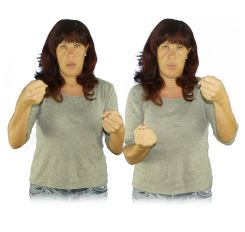
\includegraphics[width=0.5\textwidth]{Imagenes/Fuentes/Text2LSE/imagenEjemplo.jpg}
	\caption{Imagen devuelto por el servicio de traducción de la palabra \textit{``coche''} a LSE}
	\label {fig: imgCoche}
\end{figure}


\subsection{Servicio web para Traducción de texto en castellano a texto en LSE}
Este servicio implementa la funcionalidad de traducción de un texto en castellano a LSE en formato texto.
Para poder acceder a este servicio, se debe realizar una petición POST a la API en la siguiente URL:

\begin{shaded}
	\url{https://holstein.fdi.ucm.es/tfg-text2lse/TextoLSE}	
\end{shaded}


Los datos a enviar en la petición POST deben tener la siguiente estructura en JSON: 
\begin{center}
	
	\{ 'Texto' : '<texto>' \}
	
\end{center}

En el parámetro ``texto'' se debe incluir el texto que se desea traducir a LSE. Un ejemplo de uso sería: 



\begin{center}
	Entrada:  \{ ``Texto'' : ``El niño bebe agua.'' \}\\
	Salida:   \{ ``Texto'' : ``niño agua beber.'' \}
\end{center}


El flujo de este servicio web lo podremos ver en la Figura~\ref {fig: imgFlujoFlujoTextoLSE}.


\begin{figure}[]
	\centering
	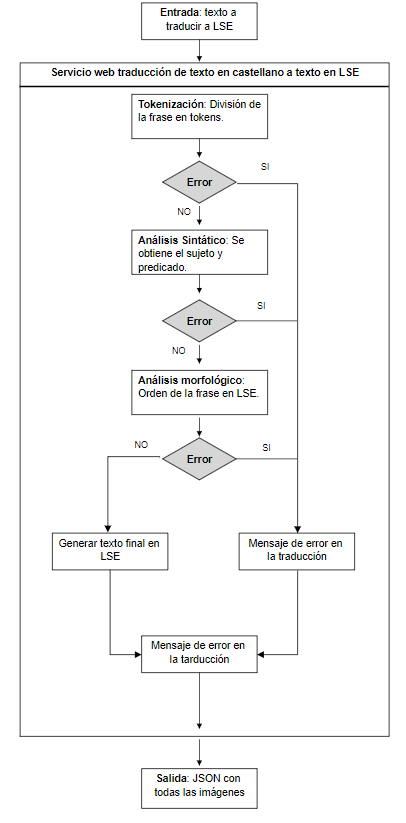
\includegraphics[width=1\textwidth]{Imagenes/Fuentes/Text2LSE/textotextoLSE.png}
	\caption{ Flujo servicio de traducción de texto en castellano a texto en LSE }
	\label {fig: imgFlujoFlujoTextoLSE}
\end{figure}

Para que el servicio web sea capaz de traducir una frase a LSE se ha tenido que realizar un procesamiento previo del texto en castellano para poder adaptarlo a la Lengua de Signos Española.


Este procesamiento es realizado con sistema de reglas las cuales filtran qué palabras deben de ser utilizadas y cuales no al igual que determina su orden en la oración en LSE. La elección a la hora de desarrollar el Procesamiento del Lenguaje Natural para nuestro proyecto estaba entre un sistema basado en reglas o mediante el uso de aprendizaje automático. La opción de desarrollar un aprendizaje automático no era viable debido a la dificultad y la falta de ejemplos en castellano para entrenar el sistema. Por este motivo se eligió el sistema basado en reglas ya que era más fácil de implementar y aunque puede limitar la capacidad de traducción de frases que no cumplan dichas reglas, cumple con los objetivos marcados en el proyecto que es traducir frases simples a LSE.\\

Nuestro PLN se divide en tres fases. Lo primero que hace es recopilar información de la frase para luego realizar un análisis sintáctico y morfológico de la frase y así poder ordenarla respetando la estructura de la LSE. A continuación se explicará con más detalle cada una de las fases:

\subsubsection{Tokenización} 
Para poder realizar el análisis sintáctico y morfológico de la frase se necesita obtener toda la información posible de la frase. Para ello se realizará el proceso de tokenización el cual divide la frase en una lista de palabras denominadas \textit{tokens} donde cada token contiene la siguiente información de cada palabra:


\begin{itemize}
	
	\item \textbf{Dependencia:} Indica la relación de dependencia sintáctica dentro de la oración, es decir, que función tiene la palabra dentro de la oración donde las más importantes son sujeto, raíz u objeto.
	\item \textbf{Tags:} Indica el género, número, el tiempo verbal y la persona de cada token.
	\item \textbf{Part of speech:} Indica el tipo de palabra en función de su uso en la oración, tales como nombres, adjetivos, adverbios y verbos.
	\item \textbf{Lemma:} Indica el lema de una palabra,es decir, la palabra que se encuentra al frente del diccionario por ejemplo, El lemma de ``jugábamos'' es ``jugar''
	
\end{itemize}


Por ejemplo los tokens que aparecen en \textit{`Los niños merendaron chocolate'} sería los que aparecen en la Figura ~\ref {fig: tokenInformacion}:
\begin{figure}[h]
	\centering
	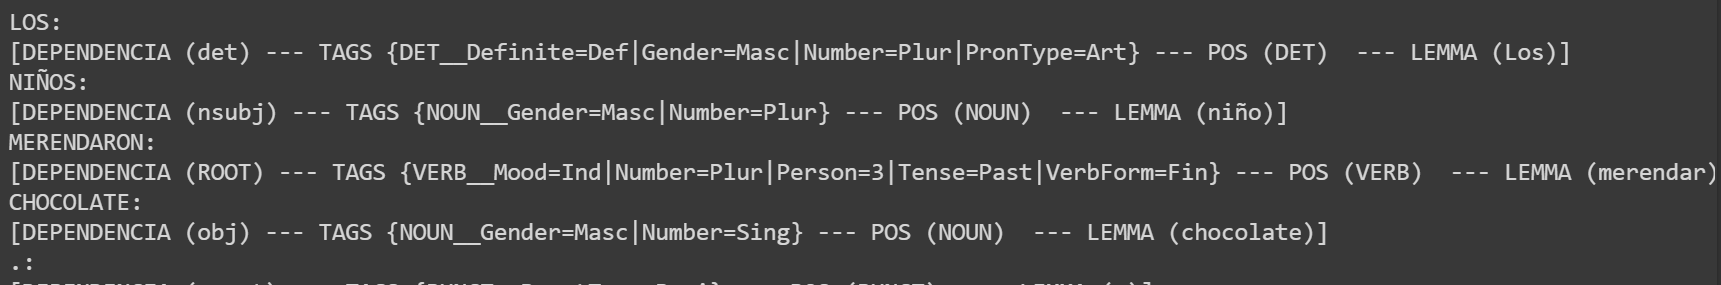
\includegraphics[width=1 \textwidth]{Imagenes/Fuentes/PNL/InfoPLN.png}
	\caption{ Tokens de la frase ``Los niños meredaron chocolate'' }
	\label {fig: tokenInformacion}
\end{figure}

Como se ve en la Figura ~\ref {fig: tokenInformacion} cada token tiene su información detallada. Por ejemplo de los tokens \textit{``los''} y \textit{``niños''} la información obtenida sería:
\begin{itemize}
		\item \textbf{Los:} la dependencia indica que es un determinante y los tags que es artículo determinado, masculino y plural. 
		\item \textbf{niños:} la dependencia indica que es el sujeto de la oración, los tags que es masculino y plural y el lemma proporciona la palabra que vendría en el diccionario.  
	
\end{itemize}
 
Mediante la tokenización a parte de poder obtener la información de cada palabra se obtiene un árbol de dependencias entre palabras. Para entender cómo funcionan las dependencias se va a utilizar como ejemplo la oración `Ayer los niños merendaban chocolate' donde sus dependencias se muestran en la Figura ~\ref {fig: dependencias} 

\begin{figure}[h]
	\centering
	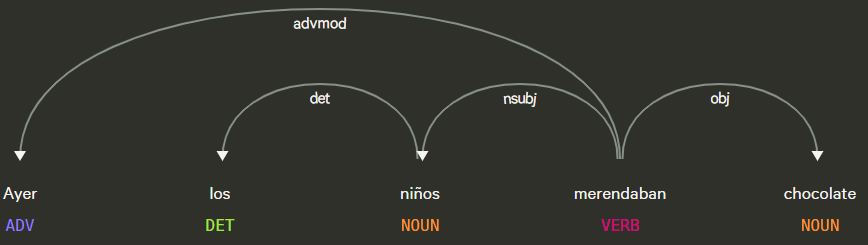
\includegraphics[width=1\textwidth]{Imagenes/Fuentes/Text2LSE/dependencias.png}
	\caption{ Displacy grafo de dependencias }
	\label {fig: dependencias}
\end{figure}

Como se puede apreciar en el diagrama del token `merendaban' dependen tres tokens (Ayer, niños y chocolate) y de ellos también dependen otros y así sucesivamente. Estas dependencias se traducen en un árbol donde el ROOT es la raíz como podemos ver en la Figura~\ref {fig: grafo}:\\


\begin{figure}[]
	\centering
	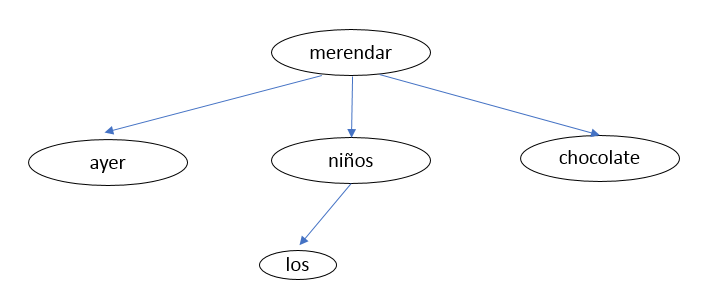
\includegraphics[width=1\textwidth]{Imagenes/Fuentes/Text2LSE/grafo.png}
	\caption{ Árbol de ls oración ``Los niños merendaron chocolate'' }
	\label {fig: grafo}
\end{figure}



\subsubsection{Análisis sintáctico} 
Una vez separado la oración en tokens hay que diferenciar que palabras forman parte del sujeto y cuales del predicado. Para ello hay que recorrer el árbol de dependencias mediante una función recursiva empezando desde el ROOT que es el token raíz del cual dependen todos los demás.\\

Para obtener el sujeto se busca el token que contenga la dependencia ``nsuj''. A continuación se obtienen los hijos del token ``nsuj'' y se guardan como parte del sujeto mientras que los tokens restantes, es decir, aquellos que no pertenecen al sujeto formarían parte del predicado. En el ejemplo anterior \textit{``Ayer los niños merendaban chocolate''} el \textbf{sujeto} sería \textit{``Los, niños''} y el \textbf{predicado} \textit{``Ayer, merendaban y chocolate''}.\\

El resultado de los tokens pertenecientes al sujeto y al predicado se almacena en una lista
\begin{center}
	\begin{itemize}
		\item \textbf{Sujeto:}  [Los, niños]
		\item \textbf{Predicado:} [Ayer, merendaban, chocolate]
		
	\end{itemize}
\end{center}

\subsubsection{Análisis morfológico} 

La Lengua de Signos Española tiene una estructura gramatical diferente al castellano. Para comenzar con la traducción se toma como punto de partida la estructura más simple en LSE: 
\begin{center}
	TIEMPO + SUJETO + OBJETO + VERBO.
\end{center}

Como se explica en la sección ~\ref {cap2:sec:Sintaxis de la Lengua de Signos} en la LSE las palabras pueden estar estructuradas de forma diferente con respecto a la oración original en castellano.


Para conseguir la traducción de la frase original en castellano a LSE se necesita un análisis morfológico que permita detectar:

\begin{itemize}
	
	\item \textbf{Determinantes:} Los determinantes se omiten a la hora de hacer la traducción \textit{por ejemplo, ``El niño come carne''} se traduce como \textit{``Niño carne comer''.}
	
	\item \textbf{Verbos copulativos:} Los verbos copulativos ser, estar o parecer se omiten a la hora de la traducción \textit{por ejemplo, ``yo soy bajo''} se traduce como \textit{``yo bajo''.}
	
	\item \textbf{Posesivos:} Los determinantes posesivos se sustituyen por pronombres personales \textit{por ejemplo, ``Mi niño es bajo''} se traduce como \textit{``yo niño bajo''.}
	
	\item \textbf{Preposiciones:} Algunas preposiciones se quitan y otras se añaden \textit{por ejemplo, ``Mi niño está en el parque''} se traduce como \textit{``yo hijo parque''.} o \textit{por ejemplo, ``yo jugaba con el perro''} se traduce como \textit{``yo perro jugar''.}
	
	\item \textbf{Adjetivos:} Los adjetivos se ponen en masculino\textit{por ejemplo, ``Mi mamá es fea''} se traduce como \textit{``yo mamá feo''.}
	
	\item \textbf{Temporalidad:} La temporalidad va al principio de la oración. \textit{por ejemplo, ``Yo comí chocolate ayer''} se traduce como \textit{``Ayer yo chocolate comer''.} Sin embargo no siempre hay adverbios de tiempo en la oración que indican la temporalidad, en este caso el tiempo viene determinado por el tiempo verbal \textit{por ejemplo, ``Yo comeré chocolate''} se traduce como \textit{``Futuro yo chocolate comer''.}
	

	
\end{itemize}


Una vez añadido y quitado las palabras el sujeto y predicado, la frase se tiene que ordenar según la estructura tiempo + sujeto + objeto + verbo por lo que el resultado final de la frase usada como ejemplo ``Los niños ayer merendaban chocolate'' sería: 

\begin{center}
	\begin{itemize}
		\item \textbf{Sujeto:}  [niños]
		\item \textbf{Predicado:} [Ayer, merendar, chocolate]
		\item \textbf{Frase ordenada:} ``Ayer niños chocolate merendar'' 
		
		
	\end{itemize}
\end{center}


\subsection{Servicio web para traducción de texto en lenguaje natural a vídeo en formato texto LSE }
\label{cap5:sec:textoLSEvideo}

Este servicio implementa la funcionalidad de traducción de un texto en castellano a LSE en formato texto en función de los vídeos existentes en el sistema. Los videos utilizados en este servicio provienen del catálogo de vídeos de LSE de la web de ARASAAC\footnote{\url{http://www.arasaac.org/videos_lse.php}}. Para poder acceder a este servicio, se debe realizar la siguiente petición POST a la API:\\

\begin{shaded}
	\url{https://holstein.fdi.ucm.es/tfg-text2lse/TextoLSEVideos/  }	
\end{shaded}


Los datos a enviar en la petición POST deben tener la siguiente estructura en JSON: 
\begin{center}
	
	\{ `Texto' : `<texto>' \}
	
\end{center}


En el parámetro \textit{``texto''} se debe incluir el texto que se desea traducir a LSE. Este flujo lo podemos observar en la Figura~\ref {fig: imgFlujoTextoVideoTextoText2LSE}.\\

Por ejemplo, para traducir el texto \textit{``Mis tías comen chocolate''} a LSE en formato texto en función de los vídeos existentes, se debe realizar la llamada POST indicada anteriormente con el siguiente JSON:


\begin{center}
	Entrada: \{ `Texto' : `Mis tías comen chocolate' \} \\
	Salida: \{ `Texto' : `YO TÍO FEMENINO PLURAL CHOCOLATE COMER' \}
\end{center}

En este caso, al no encontrar el vídeo para la palabra \textit{``tías''} busca el vídeo de esa palabra sin morfemas de género y número, en este caso busca el vídeo de la palabra \textit{``tío''} añadiendo la palabra  \textit{``FEMENINO''} para indicar el femenino y la palabra  \textit{``PLURAL''} para indicar el plural.


\begin{figure}[]
	\centering
	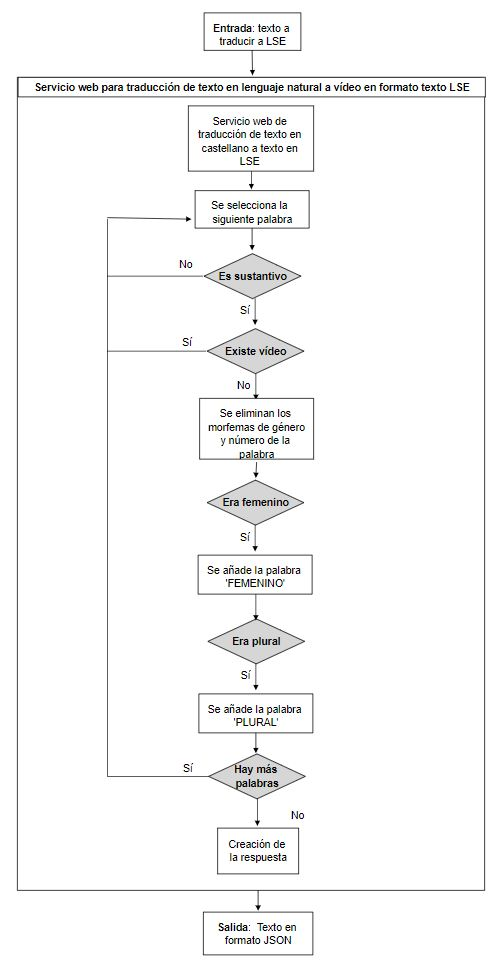
\includegraphics[width=0.8\textwidth]{Imagenes/Fuentes/Text2LSE/FlujoTextoVideoTexto.jpg}
	\caption{ Flujo servicio web para traducción de texto en lenguaje natural a vídeo en formato texto LSE }
	\label {fig: imgFlujoTextoVideoTextoText2LSE}
\end{figure}

\subsection{Servicio web para traducción de texto en lenguaje natural a imágenes en formato texto LSE}

Este servicio implementa la funcionalidad de traducción de un texto en castellano a LSE en formato texto en función de las imágenes existentes en el sistema. Las imágenes utilizados en este servicio provienen del catálogo de imágenes de LSE de la web de ARASAAC\footnote{\url{http://www.arasaac.org/signos_lse_color.php}}. Para poder acceder a este servicio, se debe realizar la siguiente petición POST a la API:\\

\begin{shaded}
	\url{https://holstein.fdi.ucm.es/tfg-text2lse/textoImagen/  }	
\end{shaded}


Los datos a enviar en la petición POST deben tener la siguiente estructura en JSON: 
\begin{center}
	
	\{ `Texto' : `<texto>' \}
	
\end{center}


En el parámetro \textit{``texto''} se debe incluir el texto que se desea traducir a LSE. Este flujo lo podemos observar en la Figura~\ref {fig: imgFlujoTextoImagenTextoText2LSE}.\\

Por ejemplo, para traducir el texto \textit{``Los caballos son rápidos''} a LSE en formato texto en función de los vídeos existentes, se debe realizar la llamada POST indicada anteriormente con el siguiente JSON:


\begin{center}
	Entrada: \{ `Texto' : `Los caballos son rápidos' \} \\
	Salida: \{ `Texto' : `CABALLO PLURAL RÁPIDO' \}
\end{center}

En este caso, al no encontrar la imagen para la palabra \textit{``caballos''} busca el vídeo de esa palabra sin morfemas de género y número, en este caso busca el vídeo de la palabra \textit{``caballo''} añadiendo la palabra  \textit{``otro''} para indicar el plural.


\begin{figure}[]
	\centering
	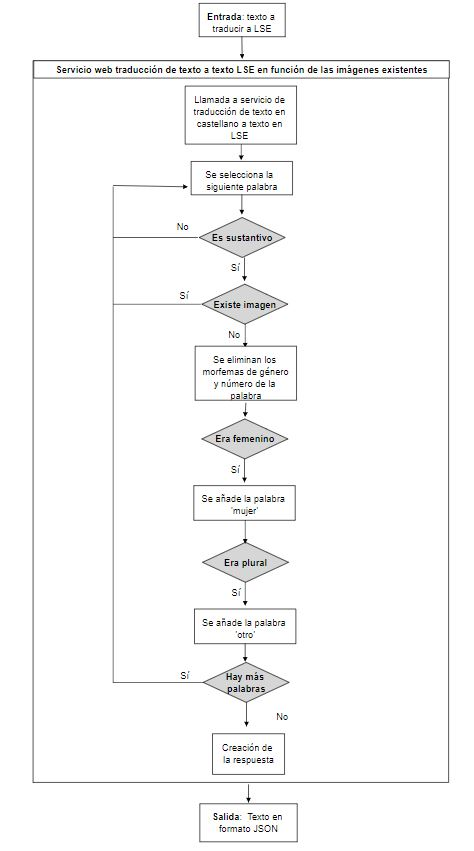
\includegraphics[width=0.8\textwidth]{Imagenes/Fuentes/Text2LSE/FlujoTextoImagenTexto.jpg}
	\caption{ Flujo servicio web para traducción de texto en lenguaje natural a imágenes en formato texto LSE}
	\label {fig: imgFlujoTextoImagenTextoText2LSE}
\end{figure}


\subsection{Servicio web para traducción de texto a LSE (vídeo)}

Este servicio implementa la funcionalidad de traducción de un texto en castellano a LSE en formato video.  Para poder acceder a este servicio, se debe realizar la siguiente petición POST a la API:\\

\begin{shaded}
	\url{https://holstein.fdi.ucm.es/tfg-text2lse/video/  }	
\end{shaded}


Los datos a enviar en la petición POST deben tener la siguiente estructura en JSON: 
\begin{center}

		\{ 'Texto' : '<texto>' \}

\end{center}


En el parámetro \textit{``texto''} se debe incluir el texto que se desea traducir a LSE. En caso de que se encuentren todos los vídeos para traducir las palabras que forman el texto solicitado en formato vídeo, se ejecuta un proceso que junta todos los vídeos en uno solo. Este vídeo es el que devuelve el servicio en formato mp4. Este flujo lo podemos observar en la Figura~\ref {fig: imgFlujoVideoTextoText2LSE}.\\

Por ejemplo, para obtener el vídeo en LSE del texto \textit{``Los niños comen chocolate''}, como podemos ver en la Figura~\ref {fig: videoOracion}, se debe realizar la llamada POST indicada anteriormente con el siguiente JSON:

\begin{center}
	
	\{ `Texto' : `Los niños comen chocolate' \}
	
\end{center}


\begin{figure}[]
	\centering
	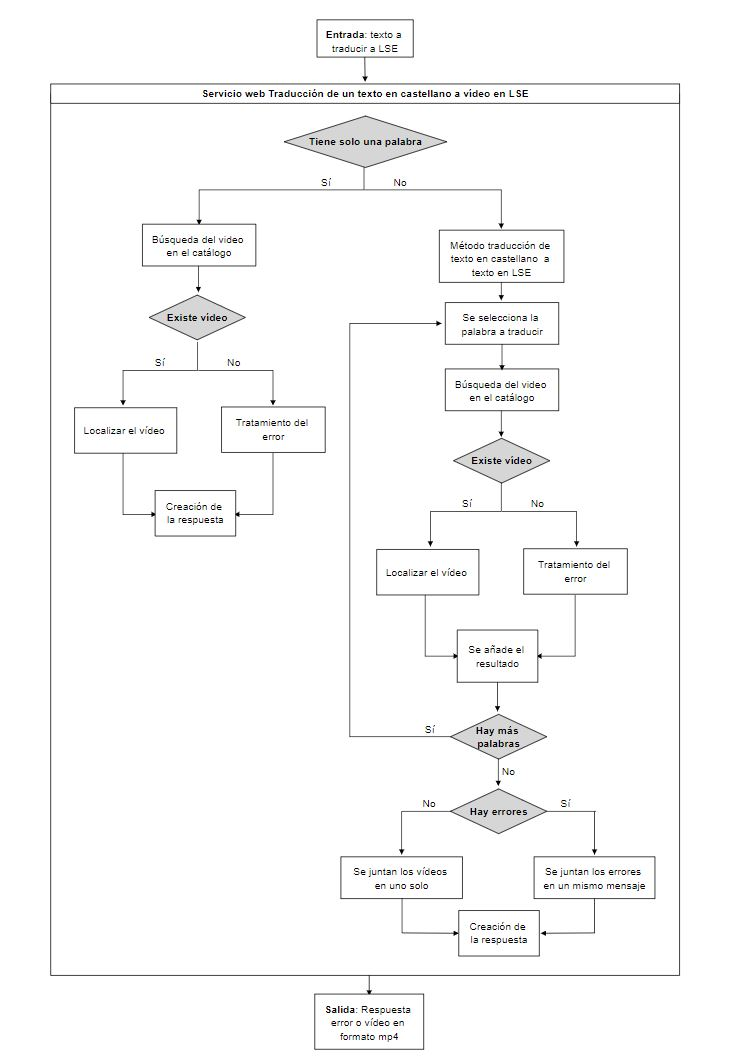
\includegraphics[width=1\textwidth]{Imagenes/Fuentes/Text2LSE/FlujoVideoTexto.jpg}
	\caption{ Flujo servicio de traducción de texto en castellano a LSE en formato vídeo }
	\label {fig: imgFlujoVideoTextoText2LSE}
\end{figure}

\begin{figure}[]
	\centering
	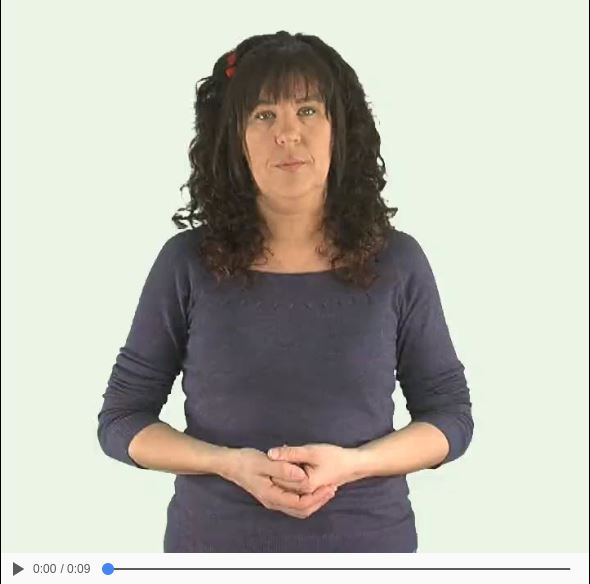
\includegraphics[width=0.5\textwidth]{Imagenes/Fuentes/Text2LSE/videoOracion.jpg}
	\caption{Vídeo devuelto por el servicio de traducción del texto \textit{``Los niños comen chocolate''} a LSE}
	\label {fig: videoOracion}
\end{figure}

El servicio web de traducción a vídeo en formato texto recibirá el texto que se desea traducir y obtendrá la traducción en texto LSE dependiendo de los vídeos disponibles. Por cada palabra de esta traducción se llamará al servicio de traducción de palabra a vídeo LSE, obteniendo así el vídeo en mp4 de todas las palabras. A continuación se concatenan todos estos vídeos, formando un único vídeo con la traducción completa que se devolverá como respuesta.\\

En caso de no existir vídeo de una o varias palabras se introducirá en su lugar un vídeo que marque el error, que se corresponde a la reproducción durante un segundo de imagen mostrada en la Figura~\ref {fig: imgError}.

\subsection{Servicio web para traducción de texto a LSE (Imágen)}
Este servicio implementa la funcionalidad de traducción de un texto en castellano a LSE en formato imagen. Las imágenes utilizadas en este servicio provienen del catálogo de imágenes de LSE de la web de ARASAAC. Para poder acceder a este servicio, se debe realizar la siguiente petición POST a la API:\\

\begin{shaded}
	\url{https://holstein.fdi.ucm.es/tfg-text2lse/imágenes/  }	
\end{shaded}

Los datos a enviar en la petición POST deben tener la siguiente estructura en JSON:

\begin{center}
	
	\{ 'Texto' : '<texto>' \}
	
\end{center}


En el parámetro \textit{``texto''} se debe incluir el texto que se desea traducir a LSE. En caso de que se encuentren los recursos para traducir las palabras solicitadas en formato imagen, se van añadiendo en un array respetando el orden de la traducción. Este array es el que devuelve el servicio en formato json. Este flujo lo podemos observar en la Figura~\ref {fig: FlujoImagenTexto}.\\

\begin{figure}[]
	\centering
	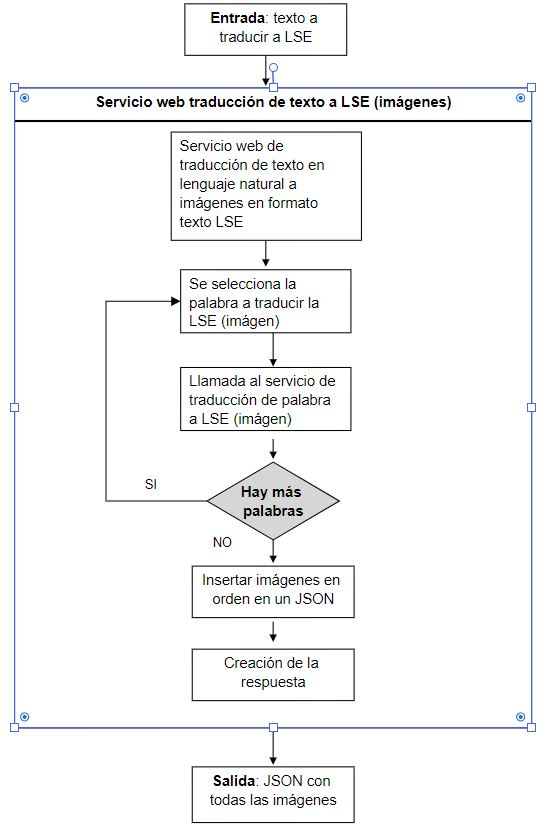
\includegraphics[width=1\textwidth]{Imagenes/Fuentes/Text2LSE/FlujoImagenTexto.jpg}
	\caption{ Flujo servicio de traducción de texto en castellano a LSE en formato vídeo }
	\label {fig: FlujoImagenTexto}
\end{figure}


\section{Front-End}

En esta sección se explica en detalle la aplicación web desarrollada, cuya finalidad es proporcionar a los usuarios una interfaz sencilla donde puedan introducir el texto que desean traducir y obtener la traducción del texto en LSE, tanto en imágenes como en vídeo. En la  Figura~\ref {fig: imgWebText2LSE} se muestra la interfaz de la aplicación, que consta de un input donde el usuario podrá introducir el texto en castellano que desee traducir, un desplegable donde podrá seleccionar el formato de salida y un botón para realizar la traducción.\\

Los formatos de salida disponibles en el desplegable son los siguientes:

\begin{itemize}

	\item \textbf{Traducción a vídeo:} tras seleccionar este formato y pulsar el botón ``traducir'', se realizará una llamada Fetch al servicio web de traducción de texto en lenguaje natural a texto LSE (ver sección \ref{cap5:sec:textoLSEvideo}), pasando por el servidor proxy, que a su vez redirigirá la petición a la API. Una función Fetch se encargará de recibir el texto resultante y de llamar por cada una de esas palabras al servicio que devuelve el video LSE correspondiente. Posteriormente se incrustan todos los vídeos en orden en el código HTML, de tal manera que se reproduce uno detrás de otro. Así, se podrá visualizar por pantalla un vídeo en el que se podrá ver a un intérprete de ARASAAC realizando los signos LSE correspondientes. En la Figura~\ref {fig: esquemaTradVideo} se puede observar el flujo para la traducción en este formato. Se ha decidido utilizar este servicio web en lugar del servicio que devuelve el vídeo completo debido a que el tiempo de respuesta es bastante más largo y a la carga de trabajo que supone para el servidor concatenar vídeos mp4 y devolverlos como respuesta.
	

	
	\item \textbf{Traducción a imágenes:} de la misma manera que en el caso de los vídeos, tras seleccionar este formato y pulsar el botón ``traducir'', se realizará una llamada Fetch  al servicio web de traducción a Texto en lenguaje natural a texto LSE, pasando por el servidor proxy, que a su vez redirigirá la petición a la API. Una función Fetch se encargará de recibir el texto resultante y de llamar por cada una de esas palabras al servicio que devuelve la imagen LSE correspondiente. Posteriormente se incrustan todas las imágenes en orden en el código HTML. En la Figura~\ref {fig: esquemaTradImagen} se puede observar el flujo para la traducción a imágenes.

	\item \textbf{Traducción a texto LSE:} tras seleccionar este formato y pulsar el botón ``traducir'' se llamará a una función Fetch que realizará una petición a la url correspondiente. En caso de éxito aparecerá por pantalla dicho texto traducido a texto LSE.En la Figura~\ref {fig: esquemaTradTexto} se puede observar el flujo para esta traducción.

\end{itemize}


\begin{figure}[]
	\centering
	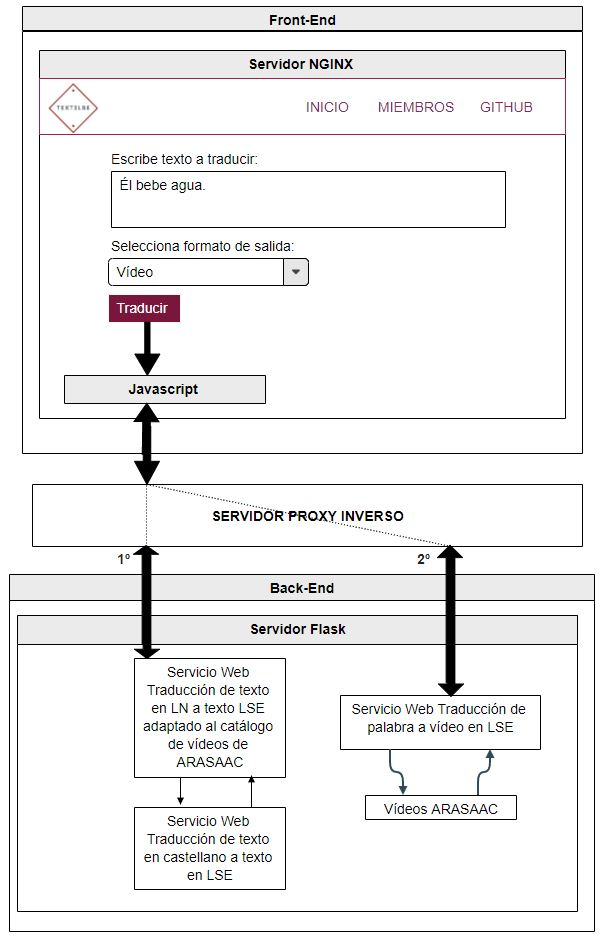
\includegraphics[width=1\textwidth]{Imagenes/Fuentes/Text2LSE/esquemaTradVideo.jpg}
	\caption{ Flujo de traducción de texto en castellano a LSE en formato vídeo }
	\label {fig: esquemaTradVideo}
\end{figure}

\begin{figure}[]
	\centering
	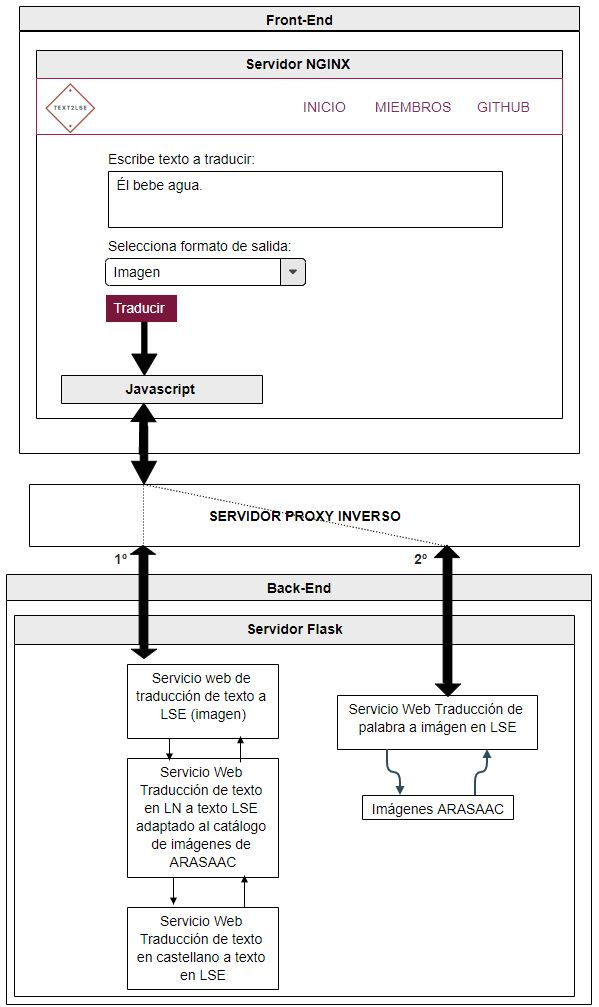
\includegraphics[width=1\textwidth]{Imagenes/Fuentes/Text2LSE/esquemaTradImagen.jpg}
	\caption{ Flujo de traducción de texto en castellano a LSE en formato imagen }
	\label {fig: esquemaTradImagen}
\end{figure}


\begin{figure}[]
	\centering
	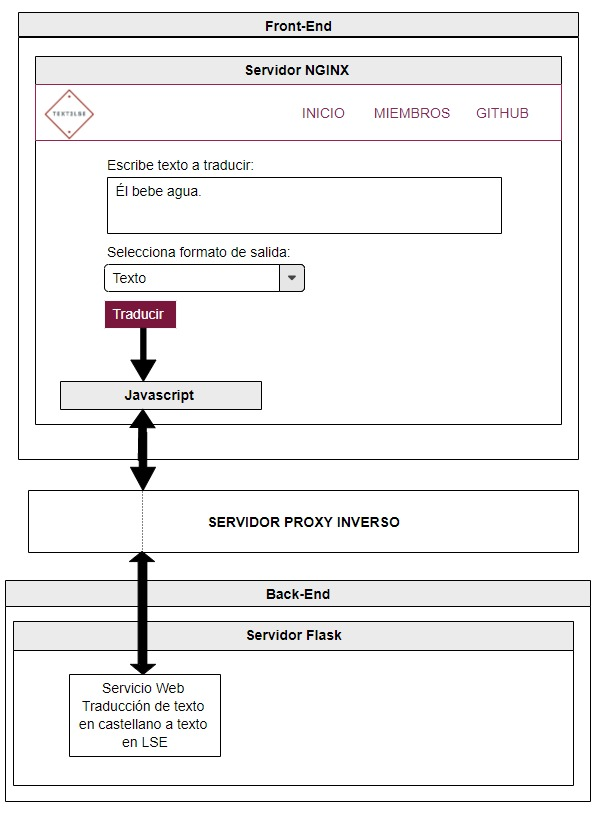
\includegraphics[width=1\textwidth]{Imagenes/Fuentes/Text2LSE/esquemaTradTexto.jpg}
	\caption{ Flujo de traducción de texto en castellano a texto LSE }
	\label {fig: esquemaTradTexto}
\end{figure}

En caso de error en cualquiera de las dos funcionalidades, la aplicación mostrará un modal con el tipo y detalle del error obtenido al realizar la petición a la API donde se encuentran nuestros servicios web.\\ 

Por otro lado, la interfaz también cuenta con un menú en la parte superior, donde además de a la página principal podemos acceder a una página con información sobre los miembros del equipo y de los tutores, y a otra con información sobre la aplicación. Todo ello se ha implementado siguiendo un diseño responsive, haciendo uso de Bootstrap 3, para garantizar que la herramienta sea accesible desde cualquier dispositivo. En la Figura~\ref {fig: imgResponsive} podemos observar la interfaz vista desde un dispositivo móvil.\\


\begin{figure}[]
	\centering
	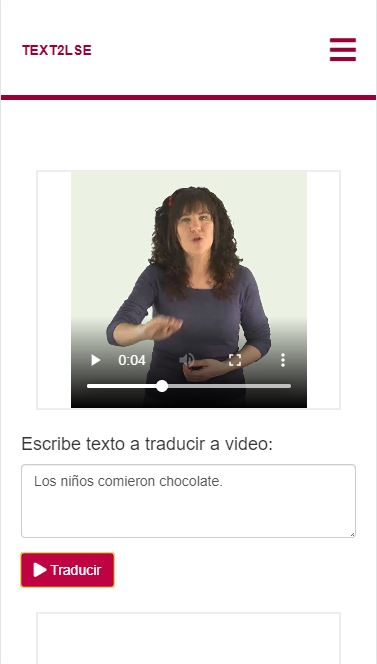
\includegraphics[width=0.75\textwidth]{Imagenes/Fuentes/Text2LSE/responsive.jpg}
	\caption{ Aplicación Web vista desde un dispositivo móvil }
	\label {fig: imgResponsive}
\end{figure}



